% Ch3.tex

\chapter[Methodology]{Methodology}
\label{cha:cha3Method}

The flowchart of a frog call classification system is depicted in Figure.~\ref{fig:flowchart}, which includes three parts: signal pre-processing, feature extraction, and classification. In this dissertation, we primarily focus on feature extraction and classification.


\section{Feature extraction}

In this section, feature extraction which always plays a key role in the classification performance is studied. A number of methods that have been used in this research for extracting relevant features of frog vocalizations are investigated.

\subsection{Introduction}

For any pattern recognition or statistical analysis, feature extraction aims to provide the most compact and informative signature for a machine learning model or classifier. Meanwhile, feature extraction is often seen as a step to facilitate the subsequent learning and generalization parts. For a classification system, it is necessary to perform feature extraction, because analysing complex data generally requires a large amount of memory and computational power. Also, a classification system without feature extraction might be caused to be over-fitting for training samples and generalize poorly to new samples.  To be specific, feature extraction consists of a number of steps as shown in Figure.~\ref{fig:feature_extraction}. To analyse different types of objects, the representation of raw data varies a lot. For instance, an audio and a video signal can be displayed using 1-Dimension representation and 2-Dimension representation, respectively.  Since the raw data are usually collected under different unconstrained environments, it is necessary to perform pre-processing to obtain efficient and distinguished features.   


\begin{figure}[htb!]
\centering
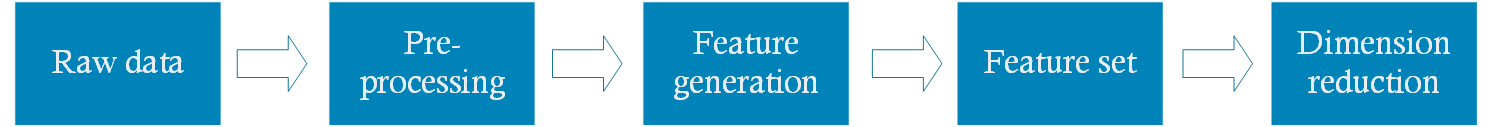
\includegraphics[width=\textwidth]{image/Method/feature_extraction.png}
\caption[Feature extraction process]{Feature extraction process}
\label{fig:feature_extraction}
\end{figure}

After pre-processing, feature generation is the next step, which directly applies various standard methods to the data. To increase the discriminability of generated features, it is also worthwhile considering the specific domain knowledge and underlying physical phenomenon. Then, feature set is constructed with the format of a scalar or vector per feature. Also the format can be one vector that concatenates all features or one matrix holding all samples of features. Finally, dimension reduction is an optional step with the following advantages: (1) reduces the time and storage space; (2) removes the multi-collinearity and improves the system performance; (3) makes it easier to visualise the data. As for the implementation of dimension reduction, there are two approaches: (1) selects a subset of the original features; (2) transforms the data into another space using the different dimensions. 

The vocalisations of frogs are innate in structure and may therefore contain indicators of phylogenetic history. Thus, frogs that are closely related phylogenetically often share similar advertisement calls.  Based on this assumption, frogs can be classified by their calls. Over the past two decades, different semi-automated and automated methods have been developed to extract features from frog calls. Most features that have been used in the previous studies are list below.

%Most features are directly transplanted from the speech and speaker domain. The descriptions of those features are list below. Several new features are developed for studying frog calls in this research, and their descriptions are list in Chapter 4 and 5.

\subsection{Various features used in the literature}

\subsubsection{Spectral centroid}
Spectral centroid (SC) is the centre point of spectrum distribution. In terms of human audio perception, it is often associated with the brightness of the sound. With the magnitude as the weight, it is calculated as the weighted mean of the frequencies.

\begin{equation}
SC=\frac{\sum_{k=0}^{N-1}f_{k}X(k)}{\sum_{k=0}^{N-1}X(k)}
\end{equation}
where $X(k)$ is the DFT of the signal syllable of the k-th sample, N is the half size of DFT. 

\subsubsection{Spectral flatness}

Spectral flatness (SF) provides a way to quantify the tonality of a sound. A high spectral flatness indicated a similar amount of power of the spectrum in all spectral bands. Spectral flatness is measured by the ratio of the geometric mean and the arithmetic mean of the power spectrum and defined as

\begin{equation}
SF = \frac{\sqrt{\frac{1}{N}\sum_{k=0}^{N-1}InX(k)}}{\frac{1}{N}\sum_{k=0}^{N-1}{X(k)}}
\end{equation}


\subsubsection{Spectral flux}


Spectral flux is used to measure how quickly the power spectrum of a signal is changing. By comparing the power spectrum between one frame and its previous one, the spectral flux can be obtained. The calculation of spectral flux is denoted as 
\begin{equation}
SX = \sum_{k=-N/2}^{N/2-1} H[|X(n,k)| - |X(n-1,k)|]
\end{equation}
where $H(x)=(x+|x|)/2$ is half-wave rectifier function.



\subsubsection{Spectral roll-off}
Spectral roll-off (SR) is often used to measure the spectral shape, and defined as the frequency H below which θ of the magnitude distribution is concentrated. 

\begin{equation}
\sum_{k=1}^{H}X(k) = \theta \sum_{k=1}^{N-1}X(k)
\end{equation}
Here $\theta$ is set at 0.85.


\subsubsection{Signal bandwidth}
Signal bandwidth ($BW$) is often used to represent the difference between the upper and lower cutoff frequencies. 

\begin{equation}
BW = \sqrt{\frac{\sum_{k=0}^{N-1}(k-SC)^{2}|x(n)|}{\sum_{k = 0}^{N-1}X(k)}}
\end{equation}


\subsubsection{Mean values for dominant frequency}
Dominant frequency (spectral peak) corresponds to the point of maximal amplitude along the frequency spectrum. Mean values for dominant frequency is defined as
\begin{equation}
MDF=\frac{\sum_{i=1}^{K}f_{i}}{K}
\end{equation}
 where $K$ is the number of frames in a frog syllable.


\subsubsection{Oscillation rate}
Oscillation rate is calculated in the frequency boundary around the fundamental frequency. First, the power within the frequency boundary is calculated. Then, the first and last 20\% part of the power vector is discarded after normalization for their uncertain. Next, the autocorrelation is applied by the length of the vector. Furthermore, a discrete cosine transform is employed to the vector after the mean subtraction, and the position of the highest frequency is achieved for calculating the oscillation rate. Detailed description can be found in our previous study \citep{Xie1504:Acoustic}.


\subsubsection{Zero-crossing rate}
Zero-crossing rate ($ZCR$) means the rate of signal change along a signal. When adjacent signals have different signs, a zero-crossing occurs. It can be defined as
\begin{equation}
ZCR = \frac{1}{2}\sum_{k=0}^{N-1}[sgn(X(k))-sgn(X(k+1))]
\end{equation}

\subsubsection{Shannon entropy}
Shannon entropy ($SEY$) is the expected information content of a sequence of signal. It describes the average of all the information contents weighted by their probabilities $p_{i}$.
\begin{equation}
SEY = -\sum_{i=1}^{L}p_{i}log_{2}(p_{i})
\end{equation}
where $L$ is the length of a frog syllable.


\subsubsection{R$\acute{e}$nyi entropy}

R$\acute{e}$nyi entropy can be used to obtain different averaging of probabilities via the parameter $alpha$, and defined as
\begin{equation}
REY=\frac{1}{1-\alpha}log_{2}(\sum_{i}^{n}p_{i}^{\alpha})
\end{equation}
where $p_{i}$ is the probabilities of the occurrence $x(n)$ in the signal.


\subsubsection{Average energy}
Average energy ($AVG$) is defined as the sum of intensity of signal.
\begin{equation}
AVG = \frac{1}{f}\sum_{k=0}^{f-1}X(k)^{2}
\end{equation}


\subsubsection{LPC}
Linear prediction coding (LPC) is often used to represent the spectral envelope of speech sound \citep{itakura1975line}. LPC coefficients can be calculated using a linear predictive filter.

\begin{equation}
X(n) = \sum_{i}^{p}a_{i}x(n-i)
\end{equation}
where $p$ is the order of the polynomial $a_{i}$. In the proposed study, 13 LPC coefficients are calculated. The value of $p$ is 12 (12th-order polynomial).

\subsubsection{MFCCs}

Mel-frequency Cepstral coefficients (MFCCs) computed based on short-time analysis are used as the baseline due to the consistency, easy implementation, and reasonable performance \ref{•}. The steps for MFCCs implementation are list as follows.

\noindent  \textbf{Step 1}: Pre-emphasis
\begin{equation}
y(n)=s(n)-\alpha s(n-1)
\end{equation}
where $s(n)$ is input frog call, a typical value for $\alpha$ is 0.95.
\\[6pt]
\noindent  \textbf{Step 2}: Framing and windowing
Each syllable is separated into frames with a length of 512 samples and an overlap of 256 samples. To reduce the discontinuity on both sides of frames, each frame is multiplied by a Hamming window.
\begin{equation}
x(n)=w(n)*y(n)
\end{equation}
where $w(n)$ is the Hamming window function.
\\[6pt]
\noindent  \textbf{Step 3}: Spectral analysis
Compute the discrete Fourier transform (DFT) of each frame of the signal. By considering 
$\omega =2\pi k/N$, the DFT of each frame of the signal is 
\begin{equation}
X(k)=\sum_{n=0}^{N-1}x(n)e_{-j\omega}
\end{equation}
Equation (16) is known as signal spectrum.
\\[6pt]
\noindent  \textbf{Step 4}: Band-pass filtering
The amplitude spectrum is then filtered using a set of triangular band-pass filters.
\begin{equation}
E_{j}=\sum_{k=0}^{N/2-1}\phi_{j}(k)A_{k}, 0 \leq j \leq J-1
\end{equation}
where J is the number of filters, $\phi_{j}$ is the $j^{th}$ filter, and $A_{k}$ is the amplitude of $X(k)$.
\begin{equation}
A_{k}=|X[k]|^{2}, 0 \leq k \leq N/2
\end{equation}
\\[6pt]
\noindent  \textbf{Step 5}: DCT
MFCCs for the $i^{th}$ frame are computed by performing DCT on the logarithm of $E_{j}$. 
\begin{equation}
C_{m}^{j} = \sum_{j=0}^{J-1}\cos(m \frac{\pi}{J}(j+0.5))log_{10}(E_{j}), 0 \leq m \leq L-1
\end{equation}
where $L$ is the number of MFCCs.

In this study, the filter bank consists of 40 triangular filters, that is  $J=40$. The length of MFCCs of each frame is $16 (L=16)$. After calculating MFCCs from each frame, the averaged MFCCs of all frames within one syllable are calculated.
\begin{equation}
f_{m}= \frac{\sum_{i=1}^{K}(C_{m}^{l})}{K}, 0\leq m \leq L-1
\end{equation}
where $f_{m}$ is the $m^{th}$ MFCCs, $K$ is the number of frames within the syllable. In the training phase, the averaging of $ f_{m}$ over all training syllables for the call of the same species is regarded as the $m^{th}$ feature value $F_{m} $. A linear normalization process is applied to get the final feature.
\begin{equation}
\hat{F}_{m}=\frac{f_{m}-f_{m}^{min}}{f_{m}^{max}-f_{m}^{max}}
\end{equation}



\subsubsection{Coefficients of variations of root-mean-square energy}
Root-mean-square energy (RMS) is computed in frequency domain, using Parseval’s theorem. It is defined as
\begin{equation}
RMS = \sqrt{\sum_{k}|\frac{X(k)}{K}|^{2}}
\end{equation}

Then, coefficients of variations can be calculated as

\begin{equation}
CVR=\sqrt{E(RMS-E(RMS))^{2}}
\end{equation} 
where E(X) denotes the average of X.

\subsubsection{Multi-stage average spectrum}
Multi-stage average spectrum (MSAS) is used to extract both the time-varying and frequency-varying features within each frog syllable. The detailed steps for the MSAS method are described as follows:

\noindent \textbf{Step 1}:   Divide all the frames of a frog syllable into 3 time stages equally. Then, reclassify the similar frames into the same stage in accordance with the forward direction of time. For example, if a frame $j$ is classified into stage $i$, the frame after frame $j$ can only be classified into stage $i$ or the stage after $i$.

\noindent \textbf{Step 2}:  Calculate the distance between the spectrum of each frame and the averaged spectrum of each stage.
\begin{equation}
d(i,j)=\sqrt{\sum_{k=0}^{L-1}[X_{j}(k)-S_{i}(k)]^{2}}
\end{equation}
where $d(i,j)$ is the distance between the $j$-th frame and the $i$-th stage, $S_{i}(k)=\sum_(j=0)^(N_{i}-1)\frac{|X_{j} (k)|}{N_{i}}$, $0 \leq k \leq N-1$, $|X_{j}(k)|$ is the amplitude spectrum of the $j$-th frame, $N_{i}$ is the total number of frames in $i$-th stage.

\noindent \textbf{Step 3}: Calculate the shortest accumulation distance from the first to the last frame and stage. 
The initial point (1,1) denotes the distance between the first frame and the first stage. Let $Acc(j,i)$ denotes the shortest accumulation distance from the initial point to point $(j,i)$ which is defined as.
\begin{equation}
Acc(i,j)=min{Acc(j-1,i)+d(j,i),Acc(j-1,i-1)+d(j,i)} 
\end{equation}
where $Acc(1,i)=d(1,j)$ for all i, the $min{X}$ operation denotes the minimum value of $X$. $Acc(j-1,i)+d(j,i)$ and $Acc(j-1,i-1)+d(j,i)$ are the two candidate paths, a and b, respectively, which are considered in the calculation of the shortest accumulation distance at the point $(j,i)$. Since one frame can only be classified into one stage, the path from point $(j,i-1)$ to $(j,i)$ is forbidden in this study.

\noindent  \textbf{Step 4}: Search for the shortest path from the final point $(N_{f},3)$ back to the initial point (1,1) along with those paths that have a shorter distance between the two candidate paths after all of the shortest accumulation distances for each frame j and each stage i have been calculated. The points on the shortest path are recorded as a sequence of coordinate $P={P(1),P(2),…,P(N_{f})}$, where $N_{f}$ is the total number of frames in a syllable. 

\noindent \textbf{Step 5}: Reclassify each frame into a new stage according to the coordinate sequence of the shortest path.

\noindent \textbf{Step 6}: Repeat steps 2 to 5 until the change in the updated shortest accumulation distance of the final point is lower than the predefined threshold. 


\begin{figure}[htb!]
\centering
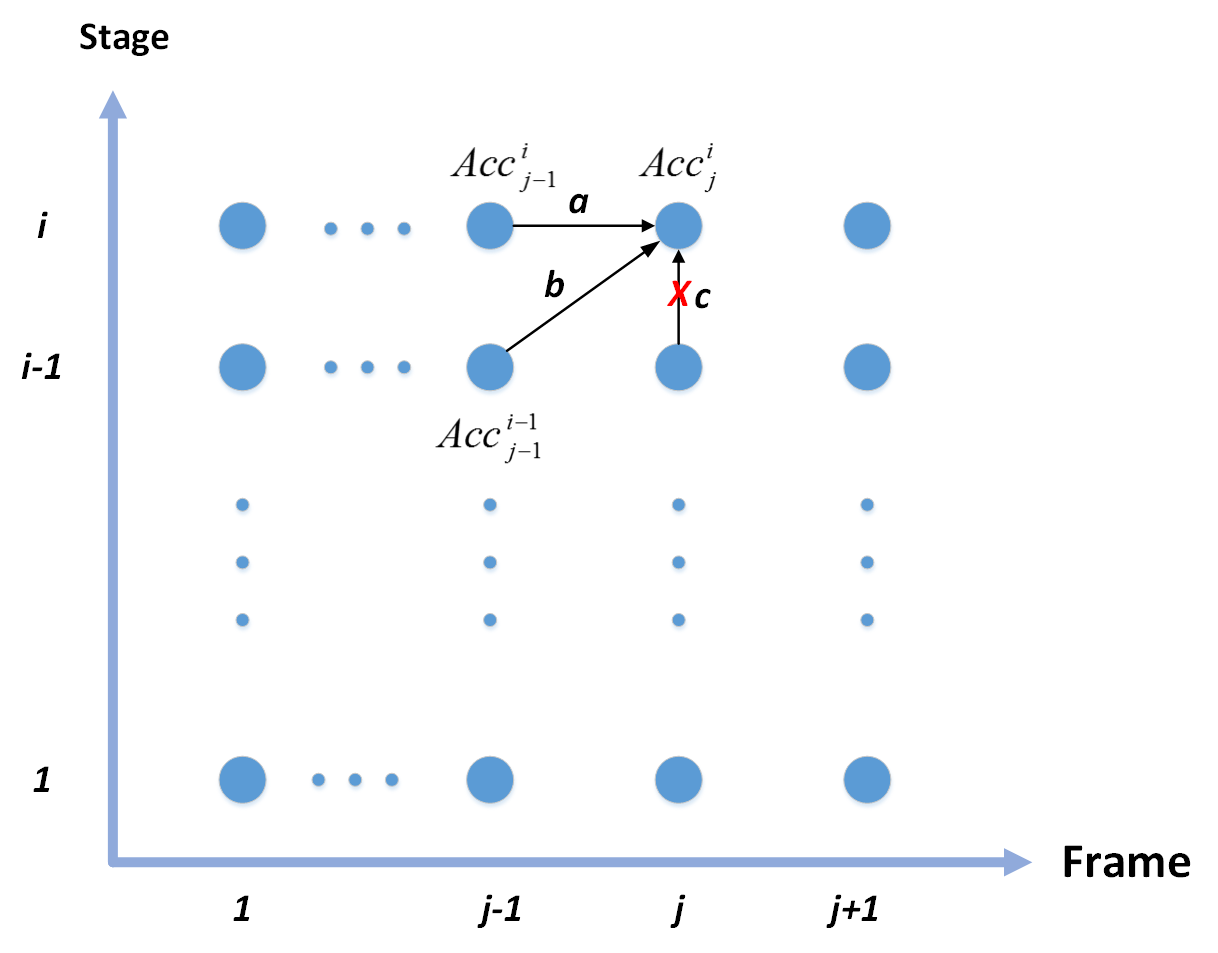
\includegraphics[width=0.75\textwidth]{image/Method/MSAS.png}
\caption[MSAS process description]{A frame and stage plane for calculating the shortest accumulation distance.}
\label{fig:flowchart}
\end{figure}

\section{Classification}


After feature extraction, the next step is to perform classification. This section aims to discuss various classification approaches used throughout this dissertation for classification of frog vocalisations. 

\subsection{Introduction}

Recent advances in acoustic sensors have made it possible to collect acoustics data over large spatial temporal scales. Also, large volumes of acoustic data are collected. Therefore, it is unavoidable to develop automatic means for data analysis. Over the past decades, machine learning has become a hot topic in the field of data analysis. Among various machine learning techniques, classification is one methodology to assign a class label to a set of unknown objects on the basis of a training data with known class membership, which is potentially useful for tagging collected acoustic data. For a classification process, it often consists of two stages: training and testing. In the training stage, a model is constructed using the testing data with known class label. In the testing stage, the learned model is used to predict the class label for the testing data. In general, classification can be divided into two types: binary classification and multiclass classification. For the binary classification, the data is separated into two classes. If the data is separated into one of several classes, then it is named as multiclass classification. Most classification methods have been specifically developed for binary classification. To extent the binary classification into multiclass classification, the combined use of multiple binary classifiers can be a solution.  For a specific classification task, it is common that several classifiers are tested in order to find a suitable classifier with high accuracy. 

\subsection{Classifiers}

\subsubsection{Linear discriminant analysis (LDA)}
LDA is a classification method originally developed in 1936 by R. A. Fisher \citep{fisher1936use}. The goal of LDA is to improve the classification accuracy at a relatively low-dimensional feature space. To achieve this goal, the within-class distance needs to be minimised while the between-class distance needs to be maximised. In LDA, a feature space from $n$-dimension to $d$-dimension can be determined by using an optimal transformation matrix, where the transformation matrix is a linear mapping that maximised the Fisher criterion.

\begin{equation}
J_{F}(\omega)=\frac{\omega^{T}S_{B}\omega}{\omega^{T}S_{W}\omega}
\end{equation}
where $S_{W}$ and $S_{B}$ are the between-class scatter matrix and within-class scatter matrix, respectively.

\begin{equation}
S_{W}=\sum_{j=1}^{C}\sum_{i=1}^{N_{j}}(X_{i}^{j}-\mu_{j})(X_{i}^{j}-\mu_{j})^{T}
\end{equation}

\begin{equation}
S_{B}=\sum_{j=1}^{C}(\mu_{j}-\mu)(\mu_{j}-\mu)^{T}
\end{equation}

where $X_{i}^{j}$ is the $i$-th vector of class $j$, $\mu_{j}$ is the mean vector of class $j$, $C$ is the number of classes, and $N_{j}$ is the number of feature vector in class $j$, $\mu$ is the mean vector of classes. 
Since LDA aims to find a transformation matrix that maximises the ratio of between-class scatter to within-class scatter in a lower-dimensional space. The optimal solution can be described as 

\begin{equation}
\omega_{opt}=argmax_{\omega}\frac{\omega^{T}S_{B}\omega}{\omega^{T}S_{W}\omega} 
\end{equation}


where transformation matrix $\omega_{opt}$ can be determined by finding the eigenvector of $S_{W}^{-1}S_{B}$.
In the recognition stage, features are first transformed into a lower-dimension by the transformation matrix $\omega_{opt}$, derived by LDA. Then the distance between the feature vector of the test data and the feature vector representing the specific class is calculated. Lastly, the one with minimum distance is regarded as the recognised class.


\subsubsection{K-nearest neighbour (K-NN)}
K-NN is a non-parametric classification method, which has been widely used for animal call classification \citep{huang2009frog, han2011acoustic, Xie1504:Acoustic, Xie2016}. An object is classified to the class of majority of its k nearest neighbours \citep{huang2009frog}.  Specifically, feature vectors are stored with class labels. For the test phase, the distances between an input feature vector and all stored vectors are calculated. Then, $k$ closest vectors are used for selecting the most frequent vector as the class label. The distance function is defined using $L^{p}$ norm, $p \in [1,\infty]$ . Here the special cases are the Manhattan distance ($p=1$), the Euclidean distance ($p=2$), and the maximum distance ($p= \infty$). The distance metric is defined as 
\begin{equation}
d_{j}^{d}=||x-x^{j}||_{p} = (\sum_{i=1}^{d}|x_{i}-x_{i}^{j}|)^{1/p}
\end{equation}

where $i$ is index of the feature vector, $j$ is the index of stored feature vector, $d$ denotes the dimension of the input feature vector. 
Next, $k$ nearest neighbours of the feature vector $i$ is selected based on the distance for selecting the most frequency vector as the class label. For instance, if the following equation satisfied 

\begin{equation}
\frac{1}{k_{1}}\sum_{j \in s_{1}}d(i,j(s_{1}) \leq \frac{1}{k_{2}}\sum_{j \in s_{2}}d(i,j(s_{2})
\end{equation}
where $k=k_{1}+k_{2}$, $k_{1}$ is the number of class $s_{1}$, $k_{2}$ is the number of class $s_{2}$. Here the input feature vector $i$ will be classified as class $s_{2}$. 



\begin{figure}[htb!]
\centering
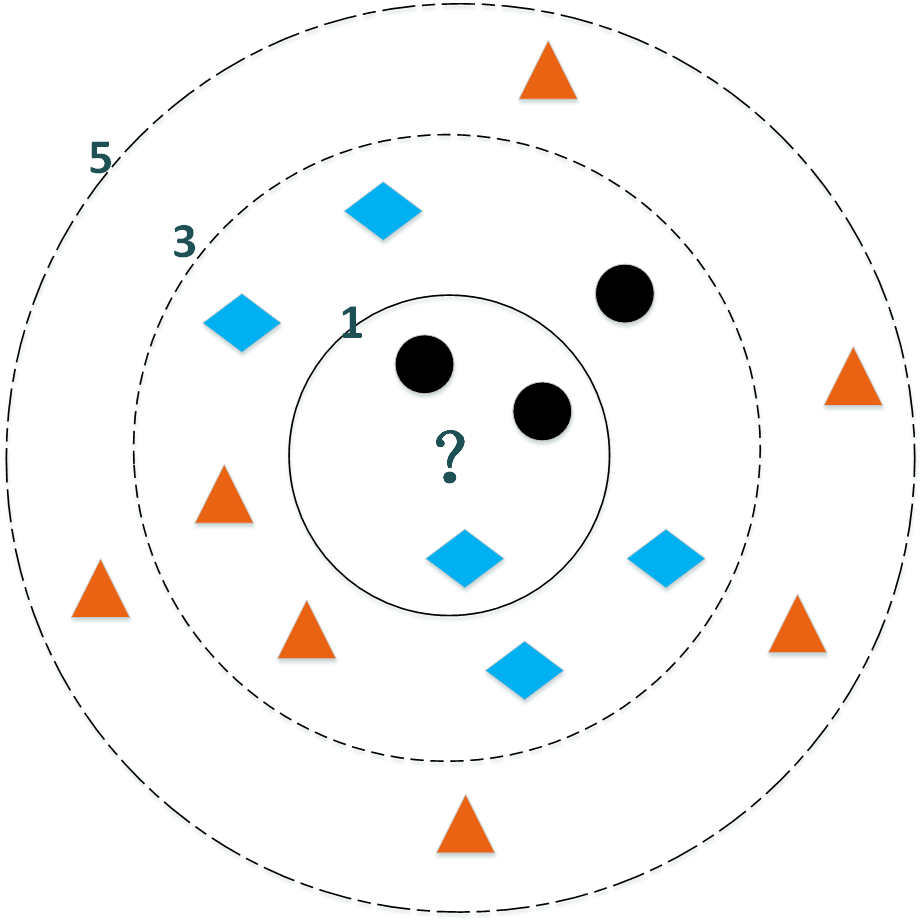
\includegraphics[width=0.6\textwidth]{image/Method/KNN.png}
\caption[A K-NN classifier]{An example of K-NN algorithm process. If $k$ is 1, then black circle will be assigned to the question mark; if $k$ is 3 then the blue diamond will be assigned to the question mark; if $k$ is 5, then green triangle will be assigned to the question mark}
\label{fig:K-NN}
\end{figure}




\subsubsection{Decision tree (DT)}


Decision tree is a tree structure that classifies instances by sorting them based on the values of feature vectors. It aims to create a model that predicts the class label of a target feature based on several input feature vectors.  Compared to other classifiers, decision tree can provide a visual representation of the classification process. Also the importance of different feature vectors is given. An example of a decision tree is shown in Figure.~\ref{fig:DT}.  For a decision tree, each internal node is labelled with an input feature, and each leaf node is labelled with a class. To construct a decision tree, an attribute value test is recursively used to split the source feature set into subsets until the subset at a node has the same value of the target variable or splitting no longer adds value to the predictions. The most common strategy for learning decision tree from data is top-down induction of decision trees \citep{quinlan1986induction}, which is an example of a greedy algorithm. 
 

\begin{figure}[htb!]
\centering
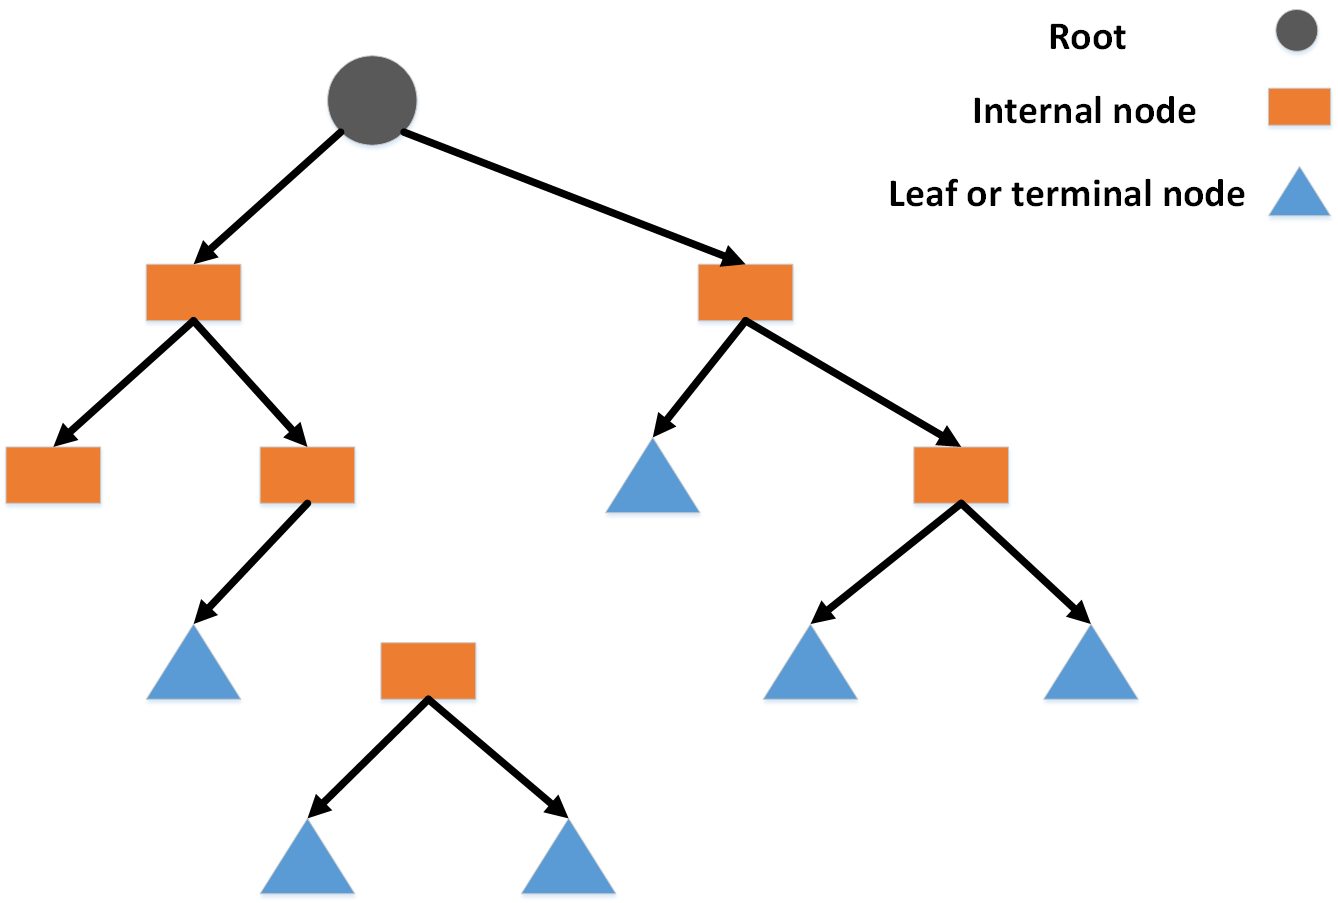
\includegraphics[width=0.75\textwidth]{image/Method/DT.png}
\caption[A DT classifier]{An example of decision tree structure with three components}
\label{fig:DT}
\end{figure}



Given a set of training instances, a feature set and cut-off value $\tau$ are used to split the data into two sets: those instances for which $X_{1}={x|x(j) \leq \tau}$ and those for which $X_{2}={x|x(j) \geq \tau}$. The choice of feature $j$ and value $\tau$ is made by minimising some measure of impurity of sets $X_{1}$ and $X_{2}$ with respect to the classes of the points in each set. A commonly used measure is the Gini index, which is defined as 

\begin{equation}
G(X)=\sum_{c \in C}p_{c}(1-p_{c})
\end{equation}
\\
where $p_{c}$ is the proportions of instances in $F$ of class $c$. The next is to find optimised feature $j$ and cutoff $\tau$ to maximise 
$G(X)-(G(X_1 )+G(X_2))$. 

\begin{equation}
(j_{opt}, c_{opt}) = argmax_{j,\tau}(G(X)-(G(X_1 )+G(X_2)))
\end{equation}
\\
where $X$ is the current set of training instances. Once the set of instances are split into sets $X_{1}$ and $X_{2}$, decision tree are recursively built on  $X_{1}$ and $X_{2}$ until some stopping criteria is met, usually a threshold of impurity or a threshold  on the minimum number of training instances in a sub-tree. 
\\
\textbf{TreeBagger}
\\
To improve performance of the decision tree algorithm and avoid over-fitting, a general technique of bootstrap aggregating or bagging is applied to tree learners \citep{breiman1996bagging}. There are two steps for this process: training and prediction.
In the training stage, a random sample with replacement of training set is repeatedly selected. Then those samples are used to train different decision trees. After training, predictions for unseen samples are made by taking the majority vote in the case of decision trees. The advantage of this bootstrapping procedure is that it decreases the variance of the model without increasing the bias.
\\
\textbf{From bagging to random forest}
\\
Based on the above bagging technique, random forest selects a random subset of the features at each candidate split in the learning process, which is sometimes called “Feature bagging” \citep{ho1995random}. The reason for doing this is the correlation of the trees in an ordinary bootstrap sample.


\subsubsection{Support vector machines (SVM)}

The support vector machine algorithm \citep{cortes1995support} often constructs a hyper-plane or set of hyper-planes in a high or infinite-dimensional space to perform classification tasks. To achieve a good classification performance, the hyper-plane is computed to have the largest distance to the nearest training-data point of any classes (maximal marginal). For a $p$-dimension data, a $(p-1)$-dimension hyper-plane is sought to separate. To explicitly explain the ideal of maximal marginal, suppose that the task is to classify data points each belong to one of two classes as shown in Figure.\ref{fig:SVM_a}. To separate the classes, there are an infinite number of lines such as $H(i),i=2,…,N-1$, but how to find the best choice ($H(N)$) based on some pre-defined requirements is the question. The reason for choosing the best line (maximal marginal) is that the one represents the best separation.  An illustration of choosing the maximum margin for data in two dimensions is given in Figure.~\ref{fig:SVM_b}. The boundaries on each side are defined by dashed lines, where the region between them is called the margin. Support vectors are defined as those data points on the boundaries.  Those data points are closest to the decision boundary (separating hyper-plane) and play the most important role in determining the margin by which are two classes are distinguished. 

Let $x_{i},i=1,\ldots ,M$ represent the training input for a binary classification task, $C_{i} \in {-1,+1}$. For the linearly separated data, the hyper-plane can then be defined as
  
\begin{figure}[htb!]
\centering
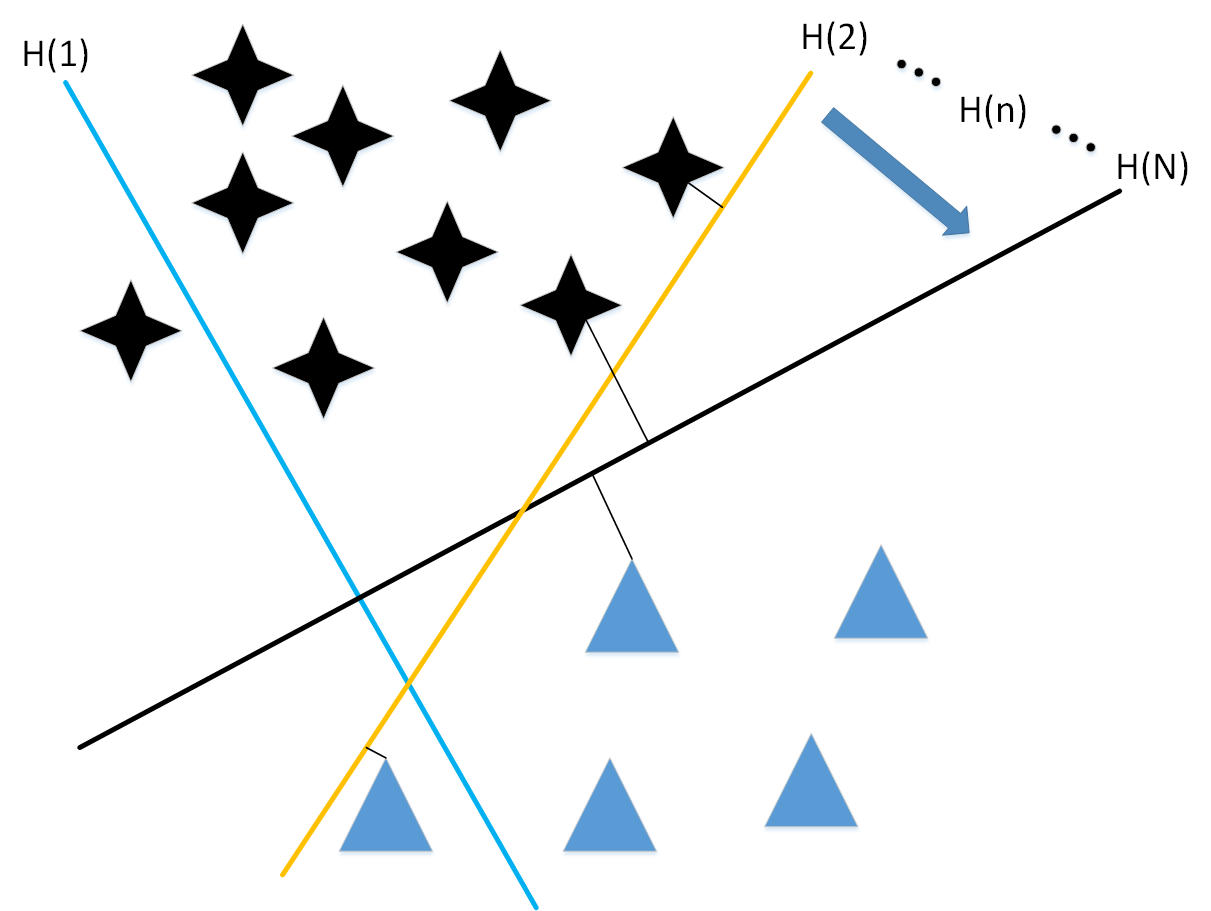
\includegraphics[width=0.7\textwidth]{image/Method/SVM.png}
\caption[A SVM classifier]{Linear separation of data for a two-class problem. Here $H(1)$ does not separate the classes; $(H(i)|i = 2:N-1)$ does, but only with a small margin; $H(3)$ separates them with the maximum margin.}
\label{fig:SVM_a}
\end{figure}
  
  
\begin{figure}[htb!]
\centering
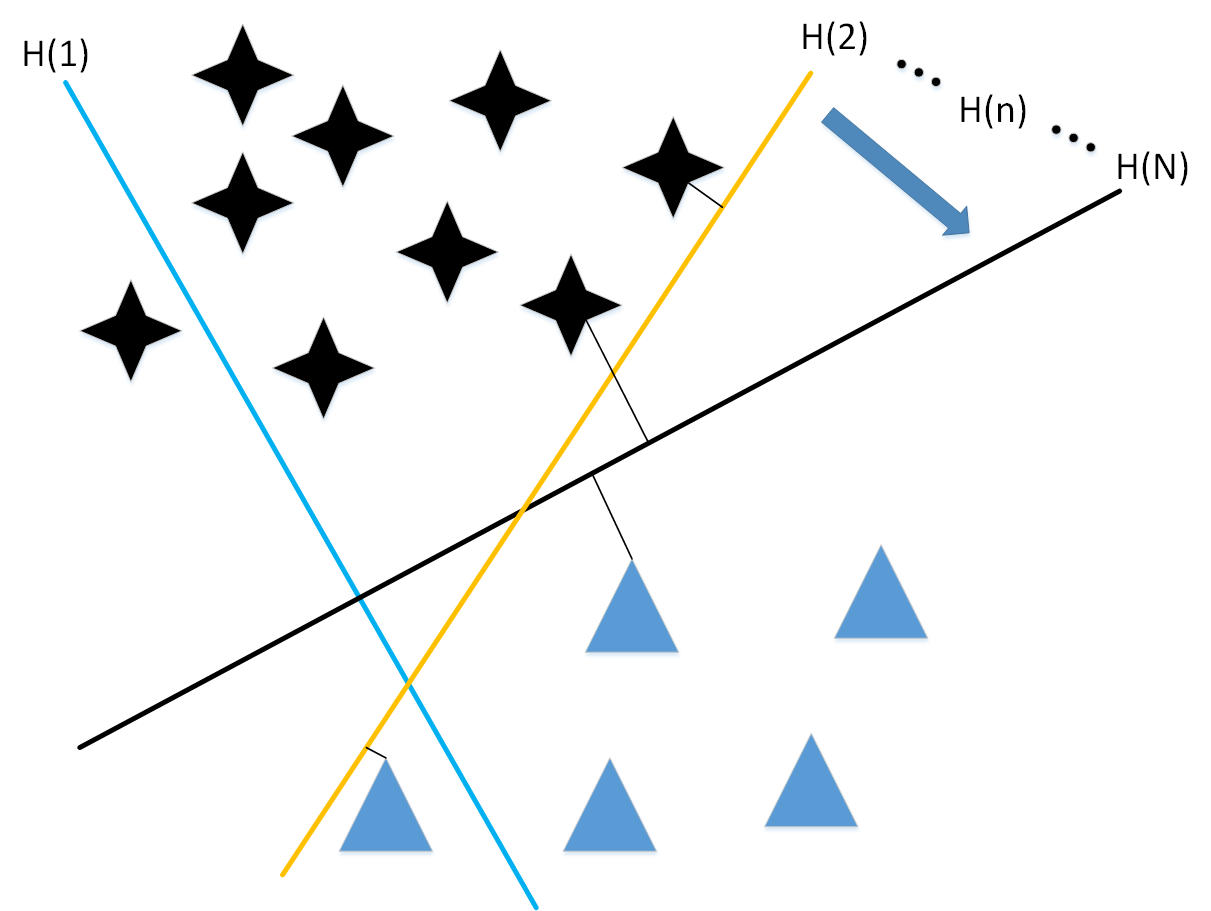
\includegraphics[width=0.7\textwidth]{image/Method/SVM.png}
\caption[A SVM classifier]{Linear separation of data using the maximum margin criteria}
\label{fig:SVM_b}
\end{figure}
  
  
\begin{equation}
D(x)=w^{T}x+b   
\end{equation}  
    
  

where $w$ is the weighting vector perpendicular to the hyper-plane, b is the scalar bias. The distance between the dashed boundary planes is inversely proportional to $||w||$ and the optimisation problem is equivalent to minimising the function

\begin{equation}
Q(w,b)=1/2||w||^{2} 
\end{equation}

Subject to the constrains that the training data satisfy
\begin{equation}
y_{i}(w^{T}x_{i}+b) \geq 1, i=1,…,M 
\end{equation}



It is possible to solve the problem with a quadratic programming algorithm when $||w||^{2}$chooses the Euclidean norm. A function of the support vectors that satisfy Eq. $3.34$ is used as the optimal hyper-plane. And it is adapt to the new training data. Therefore using standard optimisation procedures may be able to solve the minimisation problem. 

When addressing soft-margin problems where training samples are linearly inseparable, a non-negative slack variable $\xi$ is added to constraints and the object function. If $0< \xi <1$, the maximum margin does not exist in the training data. Also the aforementioned linear discriminant function may not work well for some data which in real application are corresponding features in feature space. So a non-linear kernel is introduced to map the data into a higher dimensional space by following Mercer’s theorem \citep{burges1998tutorial}. Polynomial kernel, Gaussian kernel, sigmoid kernel are some examples frequently used by researches.
The SVM algorithm is usually known as the binary classifier. A conventional remedy to make SVM possible for multi-class classification is the so called one-against-all method, which separates one class from other classes at each time. Therefore, to classify $M$ classes, the SVM algorithm needs to be run $M$ times. 


\subsubsection{Artificial neural network (ANN)}
Artificial neural network (ANN) is a non-linear, adaptive, machine learning tool built on connection principles \citep{lek1999artificial, samarasinghe2006neural}. Because of its massively parallel and distributed structure, ANN has great capabilities for learning, generalization, non-linear approximation, thus for classification. For a linear model, it is based on linear combinations of fixed non-linear basis functions $\phi_{j}(X)$ such as

\begin{equation}
y(X,W)=f(\sum_{j=1}^{W}w_{j} \phi_{j}(X))
\end{equation}
where $f(\cdot)$ is non-linear activation function in the case of classification.

For neural networks, each basis function is itself a non-linear combination of a linear combination of the inputs, where the coefficients in the linear combination are adaptive parameter.

The basis neural network model can be described as a series of functional transformations. First we construct $M$ linear combinations of the input variables $x_{1},\ldots , x_{D}$ in the form


\begin{equation}
a_{j}=\sum_{i=1}^{D}w_{ji}^{(1)}x_{i}+w_{j0}^{(0)}
\end{equation}

where $j=1, \ldots ,M$, and superscript $(1)$ indicated the corresponding parameters are in the first 'layer' of the network. The parameters $w_{ji}^{(1)}$ and $w_{j0}^{(0)}$ are used as \textit{weights} and \textit{biases}, respectively. 

The quantities $a_{j}$ are known as \textit{activations}. Then each of them is transformed using a differentiable, nonlinear activation function $h(\cdot)$ to give
\begin{equation}
z_{j}=h(a_{j})
\end{equation}

These quantities correspond to the outputs of the basis functions in Equation (3.35), which are called $hidden$ $units$ in the context of neural network.
The non-linear functions $h(\cdot)$ are generally chosen to be sigmoid functions such as the logistic sigmoid or the 'tanh' function. Then, the values are again linearly combined to give $output$ $unit$ $activations$

\begin{equation}
a_{k}=\sum_{j=1}^{M}w_{kj}^{(2)}z_{j}+w_{k0}^{(2)}
\end{equation}


where $k = 1,\ldots ,K$, and $K$ is the total number of outputs. This transformation corresponds to the second layer of the network, and again the $w_{k0}^{(2)}$ are bias parameters. Finally. the output unit activations are transformed using an appropriate activation function to give a set of network outputs $y_{k}$. The choice of activation function is determined by the nature of the data and the assumed distribution of target variables. For multiple binary classification problems, each output unit activation is transformed using a logistic sigmoid function so that

\begin{equation}
y_{k}= \sigma(a_{k})
\end{equation}
where
\begin{equation}
\sigma(a)=\frac{1}{1+exp(-a)}
\end{equation}

Combining various stages, the overall network function for sigmoid output uni activation functions can be represented as
\begin{equation}
y_{k}(X,W)=\sigma(\sum_{j=1}^{M}w_{kj}^{(2)}h(\sum_{i=1}^{D}w_{ji}^{(1)}x_{i}+w_{j0}^{(1)})+w_{k0}^{(2)})
\end{equation}
where the set of all weight and bias parameters have been grouped together into a vector $W$. Thus the neural network model is simply a non-linear function from a set of input variables ${x_{i}}$ to a set of output variables $y_{k}$ controlled by a vector $W$ of adjustable parameters.


\begin{figure}[htb!]
\centering
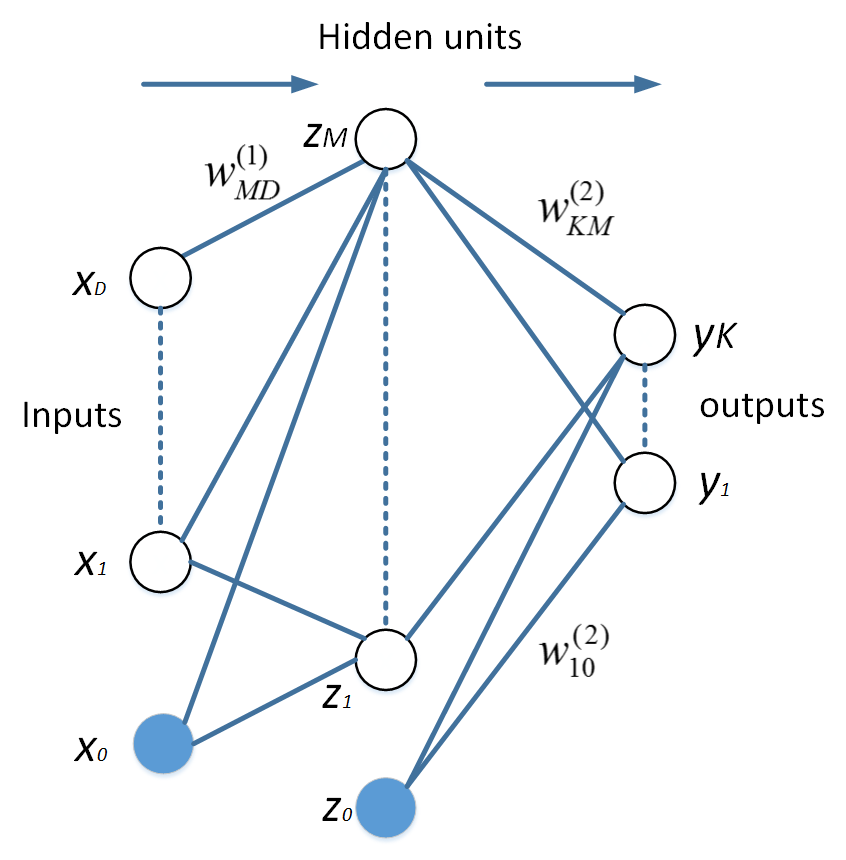
\includegraphics[width=0.7\textwidth]{image/Method/ANN.png}
\caption[An ANN classifier]{Network diagram for the two-layer neural network. The input, hidden, and output variables are represented by nodes, and the weight parameters are presented by links between the nodes. The bias parameters are denoted by links coming from additional input and hidden variables $x_{0}$ and $z_{0}$. Arrows denote the direction of information flow through the network during forward propagation}
\label{fig:ANN}
\end{figure}


\section{Conclusion}
Various feature extraction methods and classifiers (single-instance single-label) that have been used in previous studies are described. The purpose of feature representation is to represent frog vocalisations into a feature vector, which is effective enough to separate frog calls from the background noise. In high SNR recordings, most features can achieve good classification performance. However, the classification performance decreases rapidly for the environment recordings. For the classifiers, they are often designed for the classification of frog vocalisations. Since previous studies often assume that there is only one frog species in each individual recording, SISL learning is used for classification. Unfortunately, most environment recordings consists of more that one frog species. Therefore, it is worth to employ new classification frameworks to classify environment recordings with multiple simultaneously vocalising frog species.


